%%%%%%%%%%%%%%%%%%%%%%%%%%%%%%%%%%%%%%%%%%%%%%%%%%%%%%%%%%%%%%%%%%%%%
% LaTeX Template: Project Titlepage Modified (v 0.1) by rcx
%
% Original Source: http://www.howtotex.com
% Date: February 2014
% 
% This is a title page template which be used for articles & reports.
% 
% This is the modified version of the original Latex template from
% aforementioned website.
% 
%%%%%%%%%%%%%%%%%%%%%%%%%%%%%%%%%%%%%%%%%%%%%%%%%%%%%%%%%%%%%%%%%%%%%%

\documentclass[12pt]{article}
\usepackage[toc,page]{appendix}
\usepackage[a4paper]{geometry}
\usepackage[myheadings]{fullpage}
\usepackage{fancyhdr}
\usepackage{lastpage}
\usepackage{graphicx, wrapfig, subcaption, setspace, booktabs}
\usepackage[T1]{fontenc}
\usepackage[font=small, labelfont=bf]{caption}
\usepackage{fourier}
\usepackage[protrusion=true, expansion=true]{microtype}
\usepackage[english]{babel}
\usepackage{sectsty}
\usepackage{url, lipsum}
\usepackage{tgbonum}
\usepackage{hyperref}
\usepackage{array}
\usepackage[table]{xcolor}
\usepackage[utf8]{inputenc}
\usepackage{tabu}
\usepackage{listings}

\usepackage{lmodern}  % for bold teletype font
\usepackage{amsmath}  % for \hookrightarrow
\usepackage{xcolor}   % for \textcolor
\lstset{language=SQL,
basicstyle=\ttfamily,
  columns=fullflexible,
  frame=single,
  breaklines=true}


\newcommand{\HRule}[1]{\rule{\linewidth}{#1}}
\onehalfspacing
\setcounter{tocdepth}{5}
\setcounter{secnumdepth}{5}



%-------------------------------------------------------------------------------
% HEADER & FOOTER
%-------------------------------------------------------------------------------
\pagestyle{fancy}
%\fancyhf{}
%\setlength\headheight{15pt}
%\fancyhead[L]{Student ID: 1034511}
\fancyhead[R]{}
\fancyfoot[C]{Page \thepage\ of \pageref{LastPage}}
%-------------------------------------------------------------------------------
% TITLE PAGE
%-------------------------------------------------------------------------------

\begin{document}
\sloppy

{\fontfamily{cmr}\selectfont
\title{ \normalsize \textsc{}
		\\ [2.0cm]
		\HRule{0.5pt} \\
		\LARGE \textbf{\uppercase{TPC-C Database Transactions}
		\HRule{2pt} \\ [0.5cm]
		\normalsize  \vspace*{5\baselineskip}}
		}

\date{June 2019}

\author{}

\maketitle

\newpage
\tableofcontents
\newpage

%-------------------------------------------------------------------------------
% Section title formatting
\sectionfont{\scshape}
%-------------------------------------------------------------------------------

%-------------------------------------------------------------------------------
% BODY
%-------------------------------------------------------------------------------

\section{TPC-C Benchmark Guide}
\subsection{Model summary}

Understanding of the database and the structure of the Company is essential to understanding the code.

As described in Clause 1 (page 10): 

\begin{quotation}
    The Company portrayed by the benchmark is a wholesale supplier with a number of geographically distributed sales districts and associated warehouses. As the Company's business expands, new warehouses and associated sales districts are created. Each regional warehouse covers 10 districts. Each district serves 3,000 customers. All warehouses maintain stocks for the 100,000 items sold by the Company. The following diagram illustrates the warehouse, district, and customer hierarchy of TPC-C's business environment. 
    
\end{quotation}

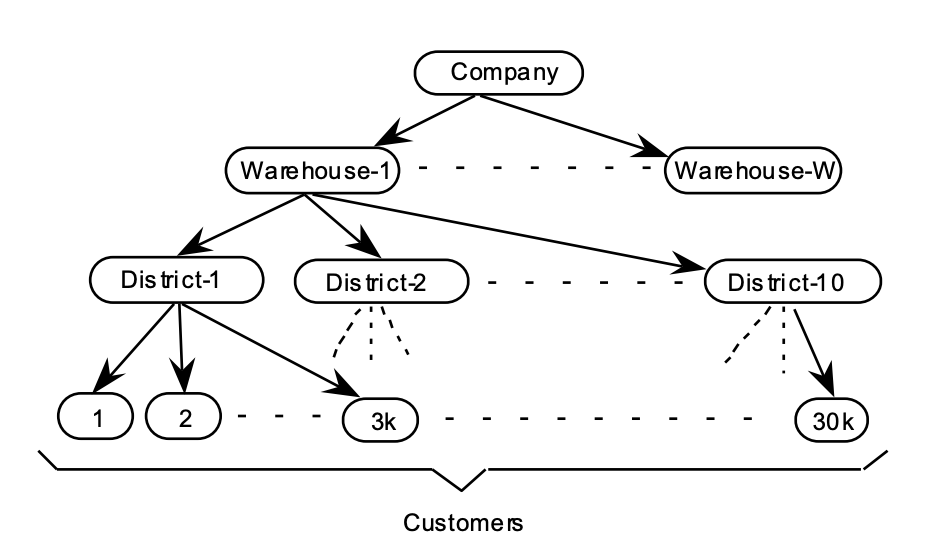
\includegraphics{img/model.png}
    
\begin{quotation}
    Customers call the Company to place a new order or request the status of an existing order. Orders are composed of an average of 10 order lines (i.e. line items). One percent of all order lines are for items not in-stock at the regional warehouse and must be supplied by another warehouse. 

    The Company's system is also used to enter payments from customers, process orders for delivery, and examine stock levels to identify potential supply shortages.
\end{quotation}

\subsection{Abridged table chema}
\textit{The TPC-C database contains nine tables. Primary keys are bolded and underlined below.}

WAREHOUSE(\underline{\textbf{wId}}, name, str1, str2, city, state, zip, tax, wYTD)

DISTRICT(\underline{\textbf{dId, wId*}}, name, str1, str2, city, state, zip, tax,  dYTD, nextOrdId)

CUSTOMER(\underline{\textbf{cId, dId, wId}}, first, middle, last, str1, str2, city, state, zip, phone, since, credit, creditLim, discount, balance, YTDPaymt, paymtCnt, deliveryCnt, data)

HISTORY(cId, cDId, cWId, dId, wId, date, amount, data)

NEWORDER(\underline{\textbf{oId, dId, wId}})

ORDER(\underline{\textbf{oId, dId*, wId*}}, cId*, entryDate, carrierId, oLCnt, allLocal)

ORDERLINE(\underline{\textbf{oId, dId*, wId*, number}}, iId, supplyWId, deliveryDate, quantity, amount, distInfo)

ITEM(\underline{\textbf{iId}}, iMId, name, price, data)

STOCK(\underline{\textbf{iId*, wId*}}, quantity, dist01, dist02, dist03, dist04, dist05, dist06, dist07, dist08, dist09, dist10, YTD, orderCnt, remoteCnt, data)



\textbf{Foreign keys:}

DISTRICT(wId) references  WAREHOUSE(wId)

CUSTOMER(wId, dId) references DISTRICT(wId, dId)

HISTORY(cWId, cDId, cId) references CUSTOMER(wId, dId, cId)

HISTORY (wId, dId) references DISTRICT(wId, dId) 

NEWORDER(wId, dId, oId) references ORDER(wId, dId, oId)

ORDER (wId, dId, cId)  references CUSTOMER(wId, dId, cId)

ORDERLINE(wId, dId, oId) references ORDER(wId, dId, oId)

ORDERLINE(supplyWId, iId) references STOCK(wId, iId)

STOCK(wId) references WAREHOUSE(wId) 

STOCK(iId) references ITEM(iId)


See Annex 1 for table cardinalities and layouts.

\section{Database generation}
\lstinputlisting{code/genDB.sql}

\section{PL/pgSQL}
PL/pgSQL is a loadable procedural language for the PostgreSQL database system. See documentation here: https://www.postgresql.org/docs/10/plpgsql-overview.html

Some notes about the PL/pgSQL syntax with regards to the functions presented in this report:

- All variables referred to in each function have to either be among the parameters of the function, or declared at the beginning of the function.

- The return type of a function must be specified at the beginning of the function. A function that returns nothing should specify with RETURNS VOID.  All of the functions below return nothing or 0, but could be modified to return desired values. 

\section{TPC-C functions}
The TPC-C document presents 5 transactions: new order (create new order), payment, order status, delivery, and stock level. The document also presents the code for a sample load program. 

\subsection{The New-Order Transaction}
\subsubsection{Overview}
The neworder function enters a complete order through a single database transaction. During the transaction, a new order is created and added into the database, the total amount to pay is calculated, and the quantity of items in stock is changed accordingly.

\subsubsection{The neworder Function}


\lstinputlisting{code/neworder.sql}

\subsubsection{The Transaction Profile}
For a given warehouse number w\_id, district number d\_id, customer number c\_id, count of items (ol\_cnt), and for a given set of items (ol\_i\_id), supplying warehouses (ol\_supply\_w\_id), and quantities (ol\_quantity):

\begin{enumerate}
    \item The row in the DISTRICT (D) table with matching D.wId and D.dId is selected, D.tax (the district tax rate) is retrieved.
    
    \item D.nextOrdId (the next available order number for the district) is retrieved and incremented by 1.
    
    \item A new row is inserted into both the ORDERS (O) and NEW\_ORDER (NO) table to reflect the creation of the new order.
    
    \item \textbf{For each item on the order (comprised of \textit{o\_ol\_cnt} items): }
    
    \begin{enumerate}
        \item The supply warehouse ID is selected from list of warehouses. If the supply warehouse ID is same as the home warehouse ID then O.allLocal is set to 1, otherwise O.allLocal is set to 0. The corresponding  values for ol\_i\_id and ol\_quantity is selected from the itemid and qty arrays.
        
        \item The row in the ITEM (I) table with matching I.iId (i.e. equals ol\_i\_id) is selected and I.price (the price of the item), I.name (the name of the item) and I.data are retrieved.
        
        \item The row in the STOCK (S) table with matching S.iId (i.e. equals ol\_i\_id) is selected and S.wId (i.e. equals ol\_supply\_w\_id) is selected. S.quantity (the quantity in stock), S.distxx (where xx represents the district number), and S.data are retrieved. The stock of the item is updated in the stock array.
        
        \item The strings in I.data and S.data are examined. If they both include the string "ORIGINAL", the brand-generic field for that item is set to "B", otherwise, the brand-generic field is set to "G".
        
        \item If the retrieved value for s\_quantity exceeds ol\_quantity then s\_quantity is decreased by ol\_quantity, otherwise s\_quantity is updated to (s\_quantity - ol\_quantity) + 91 (i.e. if not enough items are in stock to fulfill this order, then the item is restocked by 91 units before being subtracted by the quantity of items being purchased, otherwise the stock quantity of the item is subtracted by the quantity being purchased).
        
        \item ol\_amount (the amount for the item in the order) is computed as: ol\_quantity * i\_price. Adding all the items together, the total amount for the order is computed as: SUM(ol\_amount) * (1 - c\_discount) * (1 + w\_tax + d\_tax).
        
        \item A new row is inserted into the ORDERLINE table to reflect the item on the order. 
        
    \end{enumerate}
\end{enumerate}


\subsection{The Payment Transaction}
\subsubsection {Overview}

The payment business transaction updates the customer's balance and reflects the payment on the district and warehouse sales statistics. A customer can be selected by their last name or by their unique customer ID.

A Payment transaction is said to be \textbf{home} if the customer belongs to the warehouse from which the payment is entered (when CUSTOMER.wId = w\_id)

A Payment transaction is said to be \textbf{remote}if the warehouse from which the payment is entered is not the one to which the customer belongs to (when CUSTOMER.wId does not equal w\_id.

\subsubsection{The payment Function}


\lstinputlisting{code/payment.sql}

\subsubsection{The Transaction Profile}

For a given warehouse number w\_id, district number d\_id, customer number c\_id or customer last name c\_last, payment amount h\_amount, and indicator by\_name:

\begin{enumerate}
    \item The row in the WAREHOUSE (W) table with matching W.wId is selected. W.wYTD (the warehouse's year-to-date balance) is increased by h\_amount. W.name, W.str1, W.str2, W.city, and W.zip are retrieved.
    
    \item The row in the DISTRICT (D) table with matching D.wId and D.dId is selected. D.name, D.str1, D.str2, D.city, D.state, and D.zip are retrieved and D.dYtd (the district's year-to-date balance) is increased by h\_amount.
    
    \item There are two cases possible (indicated by the boolean by\_name):
    
    \begin{enumerate}
        \item \textbf{Case 1:} the customer is selected based on customer last name.
        
        All rows in the CUSTOMER (C) table with matching C.wId, C.dId and C.last are selected sorted by C.first in ascending order. Let \textit{n} be the number of rows selected. C.cId, C.first, C.middle, C.str1, C.str2, C.city, C.state, C.zip, C. phone, C.since, C.credit, C.credLim, C.discount, and C.balance are retrieved from the row at position (n/2 rounded up to the next integer) in the sorted set of selected rows from the CUSTOMER table. C.balance is decreased by h\_amount.
        
        \item \textbf{Case 2:} the customer is selected based on customer number.
        
        The row in the CUSTOMER table with matching C.wId, C.dId, and C.cId is selected. C.first, C.middle, C.last, C.str1, C.str2, C.city, C.state, C.zip, C.phone, C.since, C.credit, C.creditLim, C.discount, and C.balance are retrieved. C.balance is decreased by h\_amount.
    \end{enumerate}
    
    \item In both cases, the C.YTDPaymt is increased by h\_amount, and the C.PaymtCnt is incremented by 1.
    
    \item If the value of C.credit is equal to "BC", then C.data is also retrieved from the selected customer and the following history information: C.cId, C.dId, C.wId, D.dId, W.wId, and h\_amount, are inserted at the left of the C.data field by shifting the existing content of C.data to the right by an equal number of bytes and by discarding the bytes that are shifted out of the right side of the C.data field. The content of the C.data field never exceeds 500 characters. The selected customer is updated with the new C.data field. If C.data is implemented as two fields, they must be treated and operated on as one single field.
    
    \item The function FORMAT used in the code is similar to the C function sprintf or the Python format() function. It substitutes the placeholders in the string (the second argument) with string values of the variables that follow it.
\end{enumerate}


\subsection{The Order-Status Transaction}
\subsubsection {Overview}
The Order-Status business transaction queries the status of a customer's last order.

\subsubsection{The osstat Function}

\lstinputlisting{code/orderstatus.sql}

\subsubsection{The Transaction Profile}

For a given customer number c\_id and associated district number d\_id, warehouse number w\_id: 

\begin{enumerate}
    \item \textbf{Case 1}, the customer is selected based on customer last name: all rows in the CUSTOMER (C) table with matching C.wId, C.dId, and C.last are selected sorted by C.first in ascending order. Let n be the number of rows selected. C.balance, C.first, C.middle, and C.last are retrieved from the row at position n/2 rounded up in the sorted set of selected rows from the CUSTOMER table. 
    \item \textbf{Case 2}, the customer is selected based on customer number: the row in the CUSTOMER table with matching C.wId, C.dId, and C.last is selected and C.balance, C.first, C.middle, and C.last are retrieved.
    
    \item The row in the ORDER (O) table with matching O.wId (equals C.wId), O.dId (equals C.dId), O.cId (equals C.cId), and with the largest existing O.oId, is selected. This is the most recent order placed by that customer. O.oId, O.carrierId, O.entryDate are retrieved.
    
    \item All rows in the ORDERLINE (OL) table with matching OL.wId (equals O.wId), OL.dId (equals O.dId), and OL.oId (equals O.oId) are selected and the correspnding sets of OL.iId, OL.supplyWId, OL.quantity, OL.amount, and OL.deliveryDate are retrieved.
    
\end{enumerate}


\subsection{The Delivery Transaction}
\subsubsection {Overview}

The delivery business transaction consists of processing a batch of 10 new (not yet delivered) orders. Each order is processed (delivered) in full within the scope of a read-write database transaction. The Delivery transaction must be executed in deferred mode (more on page 40 of TPC-C document).

\subsubsection{The delivery Function}

\lstinputlisting{code/delivery.sql}

\subsubsection{The Transaction Profile}

For a given warehouse number w\_id, for each of the 10 districts d\_id within that warehouse, and for a given carrier number o\_carrier\_id: 

\begin{enumerate}
    \item The row in the NEW-ORDER (NO) table with matching NO.wId (equals w\_id) and NO.dId (equals d\_id) and with the lowest NO.oId value is selected. This is the oldest undelivered order of that district. NO.oId (the order number) is retrieved. If no matching row is found, then the delivery of an order for this district is skipped (more on page 42 of the document).
    
    \item The selected row in the NEW-ORDER table is deleted.
    
    \item The row in the ORDER (O) table with matching O.wId (equals w\_id), O.dId (equals d\_id), and O.oId (equals no\_o\_id) is selected, O.cId (the customer number) is retrieved, and O.carrierId is updated.
    
    \item All rows in the ORDER-LINE (OL) table with matching OL.wId (equals O.wId), OL.dId (equals O.dId),and OL.oId (equals O.oId) is selected. All OL.deliveryDate (the delivery dates) are updated to the current system time as returned by the operating system and the sum of all OL.amount is retrieved.
    
    \item The row in the CUSTOMER (C) table with matching C.wId (equals w\_id), C.dId (equals d\_id),and C.cId (equals O.cId) is selected and C.balance is increased by the sum of all order-line amounts (OL.amount) previously retrieved. C.deliveryCnt is incremented by 1. 
    
\end{enumerate}

\subsection{The Stock-Level Transaction}
\subsubsection {Overview}

The Stock-Level transaction determines the number of recently sold items that have a stock level below a specified threshold.

\subsubsection{The stocklevel Function}

\lstinputlisting{code/stocklevel.sql}

\subsubsection{The Transaction Profile}

For a given warehouse number (w\_id), district number (d\_id), and stock level threshold (threshold):

\begin{enumerate}
    \item The row in the DISTRICT (D) table with matching D.wId and D.dId is selected and D.nextOrdId is retrieved.
    
    \item All rows in the ORDER-LINE (OL) table with matching OL.wId (equals w\_id), OL.dId (equals d\_id), and OL.oId (lower than D.nextOrdId and greater than or equal to D.nextOrdId - 20) are selected. They are the items for 20 recent orders of the district.
    
    \item All rows in the STOCK (S) table with matching S.iId (equals OL.iId) and S.wId (equals w\_id) from the list of distinct item numbers and with S.quantity lower than threshold are counted (giving low\_stock).
\end{enumerate}

\subsection{Sample Load Program}
\subsubsection {Overview}

The code for a sample load program is given on page 117-129 of the TPC-C document. It defines the global variables, loads the tables (WAREHOUSE, DISTRICT, CUSTOMER, ORDER-LINE etc.), generates data for them according to the guidelines, and handles errors.

Worth noting are some contants and global variables used in some transactions above:

\begin{itemize}
    \item The maximum number of items: MAXITEMS = 100000
    \item Customers per district: CUST\_PER\_DIST = 3000
    \item Districts per warehouse: DIST\_PER\_WARE = 10
    \item Orders per districts: ORD\_PER\_DIST = 3000 
\end{itemize}
    



\begin{appendices}
\section{Database entities \& relationships}

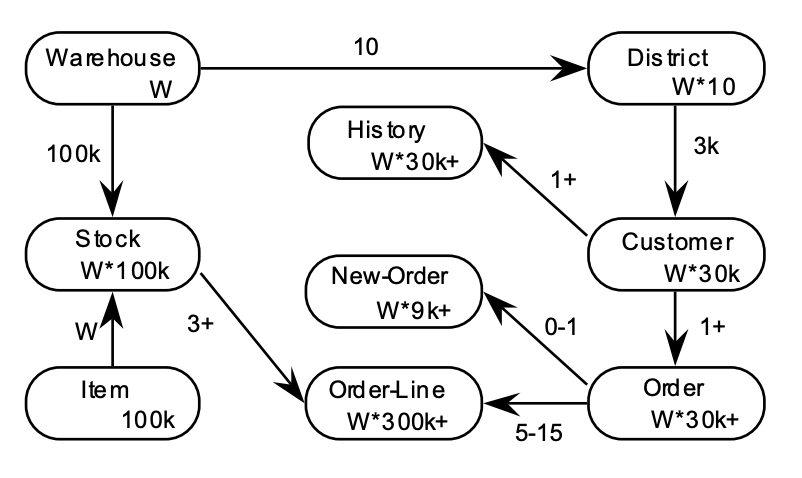
\includegraphics{img/relationships.png}

- The numbers in the entity blocks represent the cardinality of the tables (number of rows). These numbers are factored by W, the number of Warehouses, to illustrate the database scaling.

- The numbers next to the relationship arrows represent the cardinality of the relationships (average number of children per parent).

- The plus (+) symbol is used after the cardinality of a relationship or table to illustrate that this number is subject to small variations in the initial database population over the measurement interval (see Clause 5.5) as rows are added or deleted.

\section{Table layouts}

\subsection{WAREHOUSE Table Layout}

\begin{center}
\begin{tabular}{ |c|c|m{7.5cm}| } 
 \hline
 Field Name & Field Definition & Comments \\ 
 \hline
 \rowcolor{gray}
 wId & 2*W unique IDs & W Warehouses are populated \\ 
 name & variable text, size 10 &  \\ 
 str1 & variable text, size 20 & Address line 1 \\
 str2 & variable text, size 20 & Address line 2 \\
 city & variable text, size 20 &  \\
 state & fixed text, size 2 & \\
 zip & fixed text, size 9 &  \\
 tax & signed numeric(4,4) & Sales tax \\
 wYTD & signed numeric(12,2) & Year to date balance \\

 \hline
\end{tabular}
\end{center}

\subsection{DISTRICT Table Layout}

\begin{center}
\begin{tabular}{ |c|c|m{7.5cm}| } 
 \hline
 Field Name & Field Definition & Comments \\ 
 \hline
 \rowcolor{gray}
 dId & 20 unique IDs & 10 are populated per warehouse\\
\rowcolor{gray}
 wId* & 2*W unique IDs & Associated warehouse \\ 
 name & variable text, size 10 &  \\ 
 str1 & variable text, size 20 & Address line 1 \\
 str2 & variable text, size 20 & Address line 2 \\
 city & variable text, size 20 &  \\
 state & fixed text, size 2 & \\
 zip & fixed text, size 9 &  \\
 tax & signed numeric(4,4) & Sales tax \\
 dYTD & signed numeric(12,2) & Year to date balance \\
 nextOrdId & 10,000,000 unique IDs & Next available Order number, increment by 1 every time new order is added \\
 \hline
\end{tabular}
\end{center}

\subsection{CUSTOMER Table Layout}

\begin{center}
\begin{tabular}{ |c|c|m{7.5cm}| } 
 \hline
 Field Name & Field Definition & Comments \\ 
 \hline
 \rowcolor{gray}
 cId & 96,000 unique IDs & 3,000 are populated per district\\
 \rowcolor{gray}
 dId & 20 unique IDs & Associated warehouse\\
 \rowcolor{gray}
 wId & 2*W unique IDs & Customer-warehouse ID \\ 
 first & variable text, size 16 & First name\\
 middle & fixed text, size 2 & Middle initials (max 2)\\
 last & variable text, size 16 & Last name \\ 
 str1 & variable text, size 20 & Address line 1 \\
 str2 & variable text, size 20 & Address line 2 \\
 city & variable text, size 20 &  \\
 state & fixed text, size 2 & \\
 zip & fixed text, size 9 &  \\
 phone & fixed text, size 16 & \\
 since & date and time & \\
 credit & fixed text, size 2 & "GC"=good, "BC"=bad\\
 credLim & signed numeric(12, 2) & \\
 discount & signed numeric(4, 4) & \\
 balance & signed numeric(12, 2) & \\
 YTDPaymt & signed numeric(12, 2) & Customer payment year to date\\
 paymtCnt & numeric(4) & Customer payment count \\
 deliveryCnt & numeric(4) & \\
 data & variable text, size 500 & Miscellaneous information \\
 \hline
\end{tabular}
\end{center}

\subsection{HISTORY Table Layout}

\begin{center}
\begin{tabular}{ |c|c|m{7.5cm}| } 
 \hline
 Field Name & Field Definition & Comments \\ 
 \hline
 cId* & 96,000 unique IDs &\\

 cDId* & 20 unique IDs &\\

 cWId* & 2*W unique IDs & \\ 
 dId* & 20 unique IDs & \\
 wId* & 2*W unique IDs & \\ 
 date & date and time & \\
 amount & signed numeric(6, 2) & \\
 data & variable text, size 24 & Miscellaneous information \\
 \hline
\end{tabular}
\end{center}
Comment: Rows in the History table do not have a primary key as, within the context of the benchmark, there is no need to uniquely identify a row within this table. 

\subsection{NEW-ORDER Table Layout}

\begin{center}
\begin{tabular}{ |c|c|m{7.5cm}| } 
 \hline
 Field Name & Field Definition & Comments \\ 
 \hline
 \rowcolor{gray}
 oId & 10,000,000 unique IDs & \\
 dId* & 20 unique IDs &\\
 wId* & 2*W unique IDs & \\ 
 \hline
\end{tabular}
\end{center}

\subsection{ORDER Table Layout}

\begin{center}
\begin{tabular}{ |c|c|m{7.5cm}| } 
 \hline
 Field Name & Field Definition & Comments \\ 
 \hline
 \rowcolor{gray}
 oId & 10,000,000 unique IDs & \\
 \rowcolor{gray}
 dId* & 20 unique IDs & \\
 \rowcolor{gray}
 wId* & 2*W unique IDs & \\ 
 cId* & 96,000 unique IDs & \\
 entryDate & date and time & \\
 carrierId & 10 unique IDs, or null & \\
 oLCnt & numeric(2) & Count of Order-Lines (number of items) \\
 allLocal & numeric(1) & If all local then 1 else 0\\
 \hline
\end{tabular}
\end{center}

\subsection{ORDER-LINE Table Layout}

\begin{center}
\begin{tabular}{ |c|c|m{7cm}| } 
 \hline
 Field Name & Field Definition & Comments \\ 
 \hline
 \rowcolor{gray}
 oId* & 10,000,000 unique IDs & \\
 \rowcolor{gray}
 dId* & 20 unique IDs & \\
 \rowcolor{gray}
 wId* & 2*W unique IDs & \\ 
 \rowcolor{gray}
 number & 15 unique IDs & \\
 iId & 200,000 unique IDs & Item ID \\
 supplyWId & 2*W unique IDs  & \\
 deliveryDate & date and time, or null & \\
 quantity & numeric(2)  & \\
 amount & signed numeric(6, 2) & \\ 
 distInfo & fixed text, size 24 & \\
 \hline
\end{tabular}
\end{center}


\subsection{ITEM Table Layout}

\begin{center}
\begin{tabular}{ |c|c|m{7cm}| } 
 \hline
 Field Name & Field Definition & Comments \\ 
 \hline
 \rowcolor{gray}
 iId & 200,000 unique IDs  & 100,000 items are populated \\
 iMId & 200,000 unique IDs & Image ID associated to Item \\
 name & variable text, size 24 & \\
 price & numeric(5, 2) & \\
 data & variable text, size 50 & Brand information \\

 \hline
\end{tabular}
\end{center}

\subsection{STOCK Table Layout}

\begin{center}
\begin{tabular}{ |c|c|m{7cm}| } 
 \hline
 Field Name & Field Definition & Comments \\ 
 \hline
 \rowcolor{gray}
 iId & 200,000 unique IDs  & 100,000 items are populated \\
 \rowcolor{gray}
 wId & 2*W unique IDs & \\
 quantity & signed numeric(4) & \\
 dist01 & fixed text, size 24 & \\
 dist02 & fixed text, size 24 & \\
 dist03 & fixed text, size 24 & \\
 dist04 & fixed text, size 24 & \\
 dist05 & fixed text, size 24 & \\
 dist06 & fixed text, size 24 & \\
 dist07 & fixed text, size 24 & \\
 dist08 & fixed text, size 24 & \\
 dist09 & fixed text, size 24 & \\
 dist10 & fixed text, size 24 & \\
 YTD & numeric(8) & \\
 orderCnt & numeric(4) & \\
 remoteCnt & numeric(4) & \\
 data & variable text, size 50 & Information\\
 \hline
\end{tabular}
\end{center}
\end{appendices}
}
%-------------------------------------------------------------------------------
% REFERENCES
%-------------------------------------------------------------------------------
\newpage
\section*{References}

\begin{enumerate}
    
    \item TPC-C Benchmark Documentation:
    
    http://tpc.org/TPC\_Documents\_Current\_Versions/pdf/tpc-c\_v5.11.0.pdf
    
    \item PL/pgSQL Documentation:
    
    https://www.postgresql.org/docs/9.6/plpgsql.html
    
    \item Creating a function in PL/pgSQL: 
    
    https://www.postgresql.org/docs/9.1/sql-createfunction.html
    
    \item Dollar sign quotation in PL/pgSQL:
    
    https://www.postgresql.org/docs/10/sql-syntax-lexical.html#SQL-SYNTAX-CONSTANTS
    
    \item Cursors in PL/pgSQL: 
    
    https://www.postgresql.org/docs/10/plpgsql-cursors.html
\end{enumerate}

\end{document}